%!TEX root = ../report.tex

\begin{document}
    \chapter{Evaluation and Results}
    
    In this section we will report our quantitative and qualitative analysis on the results obtained from 2D Lane Detection, binary lane segmentation, followed by the resulting 3D Lane detection approaches discussed in section 4.2.3 and 4.2.6. Moreover we will discuss in detail about the current status of the proposed dual stage semi-local 3D lane detector. 
    
    \section{2D Lane Detection}
    As in our proposed approach we have adopted the dual stage way of predicting 3D lane curves inspired from \cite{guo2020gen}, where the first stage is binary lane segmentation followed by a 3D lane detector. Considering the uniqueness of the task of 2D lane detection as we need to capture rich vision cues from the environment, we stated exploring approaches like SCNN \cite{}, Ufld \cite{}, CondLaneNet \cite{}, RESA \cite{},  LaneATT \cite{}, Enet-SAD \cite{} which are performing the task of 2D Lane Detection. Though this work is mainly focused on the detecting 2D lane lines via the means of segmentation, but we have carried out a comparative evaluation of the above mentioned approaches which will form the base of experimentation for binary lane segmentation. All the above mentioned approaches were trained on  CULane \cite{} and TuSimple \cite{}. Our motive with this evaluation was to obtain the best performing segmentation based 2D lane detection architecture. We have evaluated these approaches using pre-trained models on the above mentioned datasets. The evaluation metrics used are FI score and Accuracy: 
    
    \begin{equation}
        F1 = \frac{2*precision * recall}{precision + recall}
    \end{equation}
    
where, $precision = \frac{TP}{TP + FP}$ and recall= $precision = \frac{TP}{TP + FN}$. Like in case of CULane \cite{} dataset each lane is composed of 30-pixel width and IoU(Intesection Over Union) is calculated between the predictions and and ground-truth. If IoU > 0.5, it is treated as TP. 
For TuSimple dataset accuracy is used as an offical metric to evaluate an approach which can be defined as, $accuracy = \sum_{clip} C_{clip} / \sum_{clip} C_{clip}$. Where $S_{clip}$ represents the total number of points in the clip and $C_{clip}$ is the total number of points predicted correctly. 

\begin{table}[]
 \caption{Comparative evaluation of the above mentioned approaches for the task of 2D Lane Detection}
\begin{tabular}{|c|c|c|c|c|c|}
\hline
\textbf{Approach} & \textbf{Backbone}                                                   & \textbf{Dataset} & \textbf{\begin{tabular}[c]{@{}c@{}}Pretrained \\ Metric\end{tabular}} & \textbf{\begin{tabular}[c]{@{}c@{}}Reported \\ Metric\end{tabular}} & \textbf{\begin{tabular}[c]{@{}c@{}}FPS\\ (Pre-trained \\ \& Reported)\end{tabular}} \\ \hline
SCNN              & Resnet50                                                            & CULane           & F1: 74.89                                                             & —                                                                   & —                                                                                   \\ \hline
SCNN              & \begin{tabular}[c]{@{}c@{}}LargeFOV\\ (Deep lab VGG16)\end{tabular} & CULane           & —                                                                     & F1: 71.7                                                            & —                                                                                   \\ \hline
SCNN              & Resnet18                                                            & TuSimple         & Acc: 96.05                                                            & Acc: 96.53                                                          & —                                                                                   \\ \hline
Ufld              & Resnet18                                                            & CUlane           & F1: 69.47                                                             & F1: 68.4                                                            & \textbf{$\sim$300fps}                                                               \\ \hline
Ufld              & Resnet34                                                            & CUlane           & —                                                                     & F1: 72.3                                                            & $\sim$300fps                                                                        \\ \hline
Ufld              & Resnet18                                                            & TuSimple         & Acc: 95.86                                                            & Acc:95.87                                                           & $\sim$300fps                                                                        \\ \hline
Ufld              & Resnet34                                                            & TuSimple         & —                                                                     & Acc:96.06                                                           & $\sim$300fps                                                                        \\ \hline
CondLaneNet       & Resnet101                                                           & CULane           & \textbf{F1: 79.48}                                                    & \textbf{F1: 79.48}                                                  & —                                                                                   \\ \hline
CondLaneNet       & Resnet34                                                            & CULane           & F1: 78.74                                                             & F1: 78.74                                                           & —                                                                                   \\ \hline
CondLaneNet       & Resnet18                                                            & CULane           & F1: 78.14                                                             & F1: 78.14                                                           & —                                                                                   \\ \hline
CondLaneNet       & Resnet101                                                           & TuSimple         & \textbf{Acc: 97.24}                                                   & \textbf{Acc: 97.24}                                                 & —                                                                                   \\ \hline
CondLaneNet       & Resnet34                                                            & TuSimple         & Acc: 96.98                                                            & Acc: 96.98                                                          & —                                                                                   \\ \hline
RESA              & ResNet50                                                            & CULane           & F1:75.92                                                              & F1: 75.3                                                            & $\sim$35 fps                                                                        \\ \hline
RESA              & VGG16                                                               & CULane           & —                                                                     & F1: 73.3                                                            & —                                                                                   \\ \hline
RESA              & Resnet34                                                            & CULane           & F1: 75.85                                                             & F1: 74.5                                                            & $\sim$45 fps                                                                        \\ \hline
RESA              & Resnet34                                                            & TuSimple         & Acc: 96.86                                                            & Acc: 96.82                                                          & $\sim$45 fps                                                                        \\ \hline
RESA              & Resnet18                                                            & TuSimple         & Acc: 96.73                                                            & Acc: 96.70                                                          & $\sim$47 fps                                                                        \\ \hline
LaneATT           & Resnet18                                                            & CULane           & F1: 75.10                                                             & —                                                                   & —                                                                                   \\ \hline
LaneATT           & MobileNetv2                                                         & CULane           & F1: 75.10                                                             & —                                                                   & —                                                                                   \\ \hline
LaneATT           & MobileNetv2                                                         & TuSimple         & Acc: 95.66                                                            & —                                                                   & —                                                                                   \\ \hline
LaneATT           & Resnet34                                                            & TuSimple         & Acc: 95.81                                                            & —                                                                   & —                                                                                   \\ \hline
Enet-SAD          & Resnet18                                                            & TuSimple         & (pipeline available)                                                  & Acc: 96.02                                                          & —                                                                                   \\ \hline
Enet-SAD          & Resnet18                                                            & TuSimple         & (pipeline available)                                                  & Acc: 96.24                                                          & —                                                                                   \\ \hline
Enet-SAD          & Enet                                                                & TuSimple         & (pipeline available)                                                  & Acc: 96.64                                                          & —                                                                                   \\ \hline
Enet-SAD          & Resnet18                                                            & CULane           & (pipeline available)                                                  & F1: 70.5                                                            & —                                                                                   \\ \hline
Enet-SAD          & Resnet34                                                            & CULane           & (pipeline available)                                                  & F1: 70.7                                                            & —                                                                                   \\ \hline
Enet-SAD          & Resnet101                                                           & CULane           & (pipeline available)                                                  & F1: 71.8                                                            & —                                                                                   \\ \hline
Enet-SAD          & Enet                                                                & CULane           & (pipeline available)                                                  & F1: 70.8                                                            & —                                                                                   \\ \hline
\end{tabular}
\end{table}
From the table 5.1 we can see that, CondLaneNet \cite{} performs the best on TuSimple and CULane dataset for the task of lane segmentation. As in our work we are focusing on detecting 2D lanes via the approaches which are segmentation based. Therefore our pipeline for binary segmentation, as mentioned in section 4.1 is composed of mix and match of different back-backbone, feature aggregator and heads utilized by SCNN \cite{} and \RESA{}. 
    
    
    \section{Binary Lane Segmentation}
    Binary Lane Segmentation can be seen as a sub-task of 2D lane segmentation, where instead of predicting multiple labels for different lanes we are just focusing on separating the 2D lane lines from the back ground in an image. Below we will discuss in detail the experimentation that is conducted to obtain an efficient 2D binary lane segmentation algorithm. Initially the models are trained on CULane \cite{}, TuSimple \cite{} and Apollo Synthetic dataset (sim3D) \cite{} with Cross Entropy loss as our objective function. 
    
          
    \begin{table}[h!]
    \caption{Results for binary lane segmentation using Cross Entropy loss as the loss function}
    \centering
    \begin{tabular}{|l|l|l|}
    \hline
        \textbf{Method} & \textbf{IoU} & \textbf{FPS} \\ \hline
        SCNN(Res18+TuSimple) & 54.81 & $\approx$ \textbf{70}  \\ \hline
        RESA(Res18+TuSimple) & 56.73 & $\approx$ 50 \\\hline
        SCNN(Res18+CUlane) & 38.1 & $\approx$ 70 \\ \hline
        RESA(Res18+CUlane) & 43.23 &  $\approx$ 45\\\hline
        SCNN(Res18+sim3d) & 44.12 & $\approx$ 70 \\ \hline
        RESA(Res18+sim3d) & 71.79 & $\approx$ 45 \\ \hline
        RESA(Res50+sim3d) & \textbf{74.11} & $\approx$ 40 \\ \hline
        
    \end{tabular}
\end{table}
    
       \begin{figure}[h]
       \caption{Initial binary lane segmentation results: (a) SCNN (Res18+CULane), (b) SCNN (Res18 + TuSimple) and (c) RESA (Res18 + sim3d)}
        \centering
        \begin{subfigure}{0.6\textwidth}
        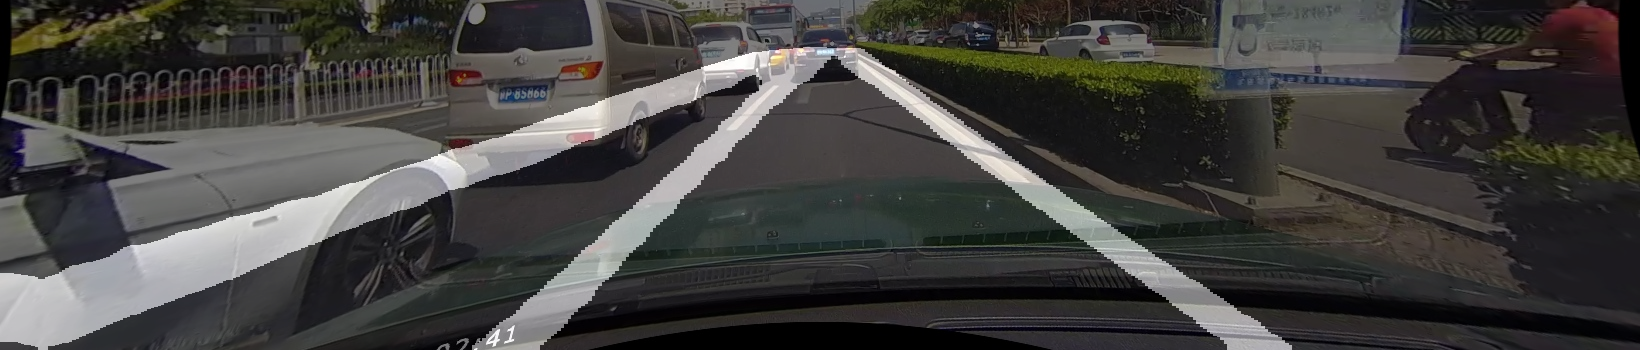
\includegraphics[width=1.2\linewidth, height=3cm]{images/SCNN_res_culane.png} 
        \caption{}
        \label{fig:subim1}
        \end{subfigure}
        \begin{subfigure}{0.4\textwidth}
        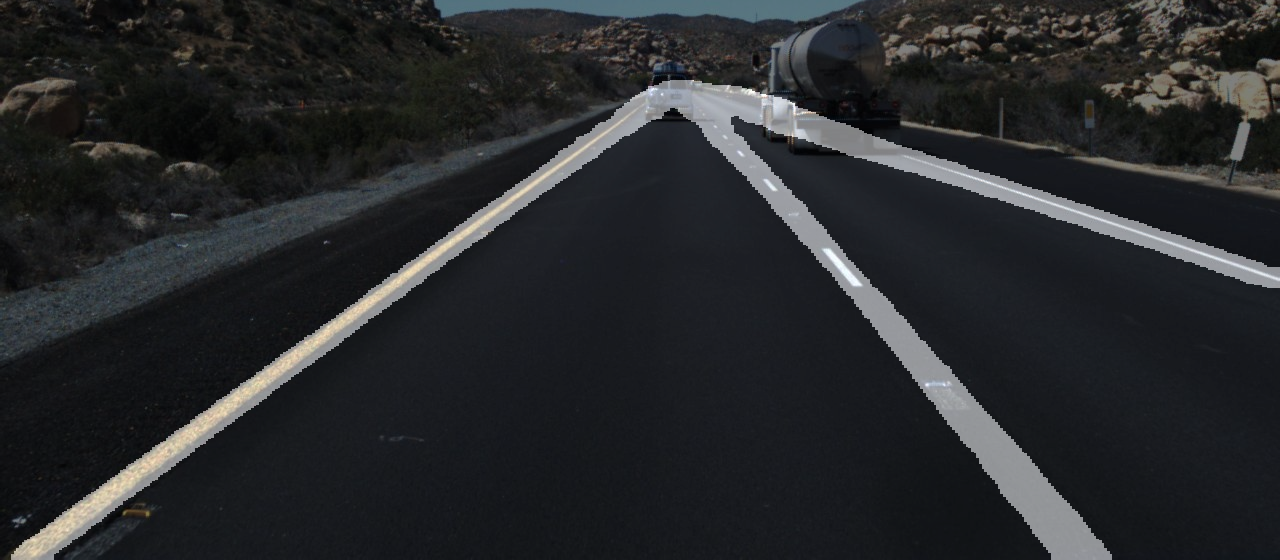
\includegraphics[width=1\linewidth, height=4cm]{images/SCNN_res_tusimple.png}
        \caption{}
        \label{fig:subim2}
        \end{subfigure}
        \begin{subfigure}{0.4\textwidth}
        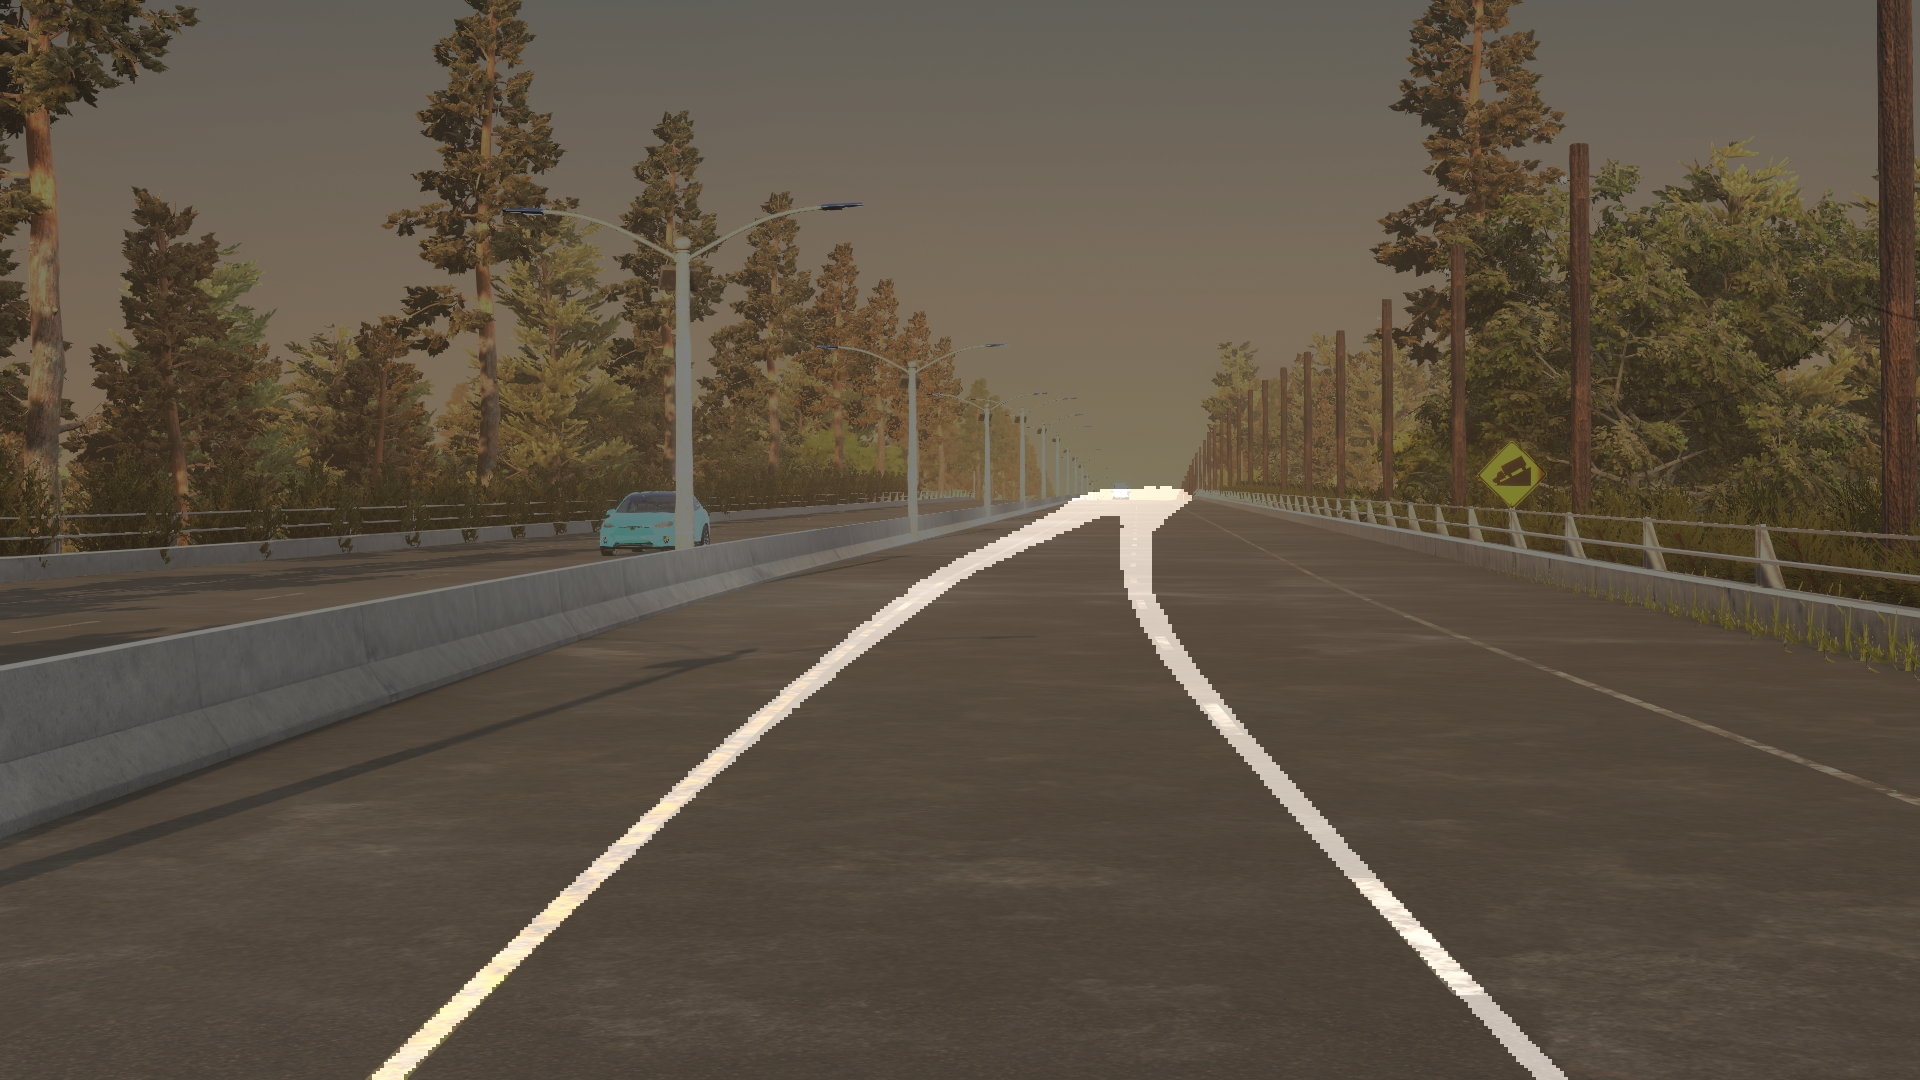
\includegraphics[width=1\linewidth, height=4cm]{images/Resa_r18_sim3d.png}
        \caption{}
        \label{fig:subim2}
        \end{subfigure}
        \label{fig:image2}
        \end{figure}
    
    From the equation \textbf{XXX} Cross entropy aims at reducing the pixel-wise error, therefore cross entropy only considers loss locally not globally. Thus the statistical distribution of labels can affect the overall loss. The cases where the occurrence of one class overpowers the other this condition is called class imbalance. Binary lane segmentation also suffers with the same problem as the number of pixels occupied by lane lines is far lesser than the number of pixels represented by the background. 
    
    Addressing this issue of class imbalance in binary lane segmentation we conducted some experiments by replacing Cross Entropy loss by Dice loss and Focal loss. Detailed explanation of these losses are mentioned in section 4.1.2. We first try to predict the 
    
     \begin{table}[h!]
    \caption{Quantitative results for binary lane segmentation trained on sim3d \cite{} dataset using Cross Entropy Loss, Focal Loss and Dice Loss}
    \centering
    \begin{tabular}{|l|l|l|}
    \hline
        \textbf{Method} & \textbf{IoU} & \textbf{FPS} \\ \hline
        RESA(Res18+Cross Entropy) & 71.79 & $\approx$ 45 \\ \hline
        SCNN(Res18+Cross Entropy) & 44.12 & $\approx$ \textbf{70}  \\ \hline
        RESA(Res50+Cross Entropy) & 74.11 & $\approx$ 40  \\ \hline
        RESA(Res18+Focal Loss) & 75.59 & $\approx$ 55 \\\hline
        RESA(Res18+Dice Loss) & 82.57 & $\approx$ 50 \\\hline
        RESA(Res50+Dice Loss) & \textbf{83.33} & $\approx$ 50 \\\hline
    \end{tabular}
\end{table}
    
      \begin{figure}[h]
       \caption{Qualitative results for binary lane segmentation trained on sim3d dataset: (a) RESA(Res18+Cross Entropy Loss) (b) RESA(Res18+Dice Loss) (c)RESA(Res18+Focal Loss)}
        \centering
        \begin{subfigure}{0.4\textwidth}
        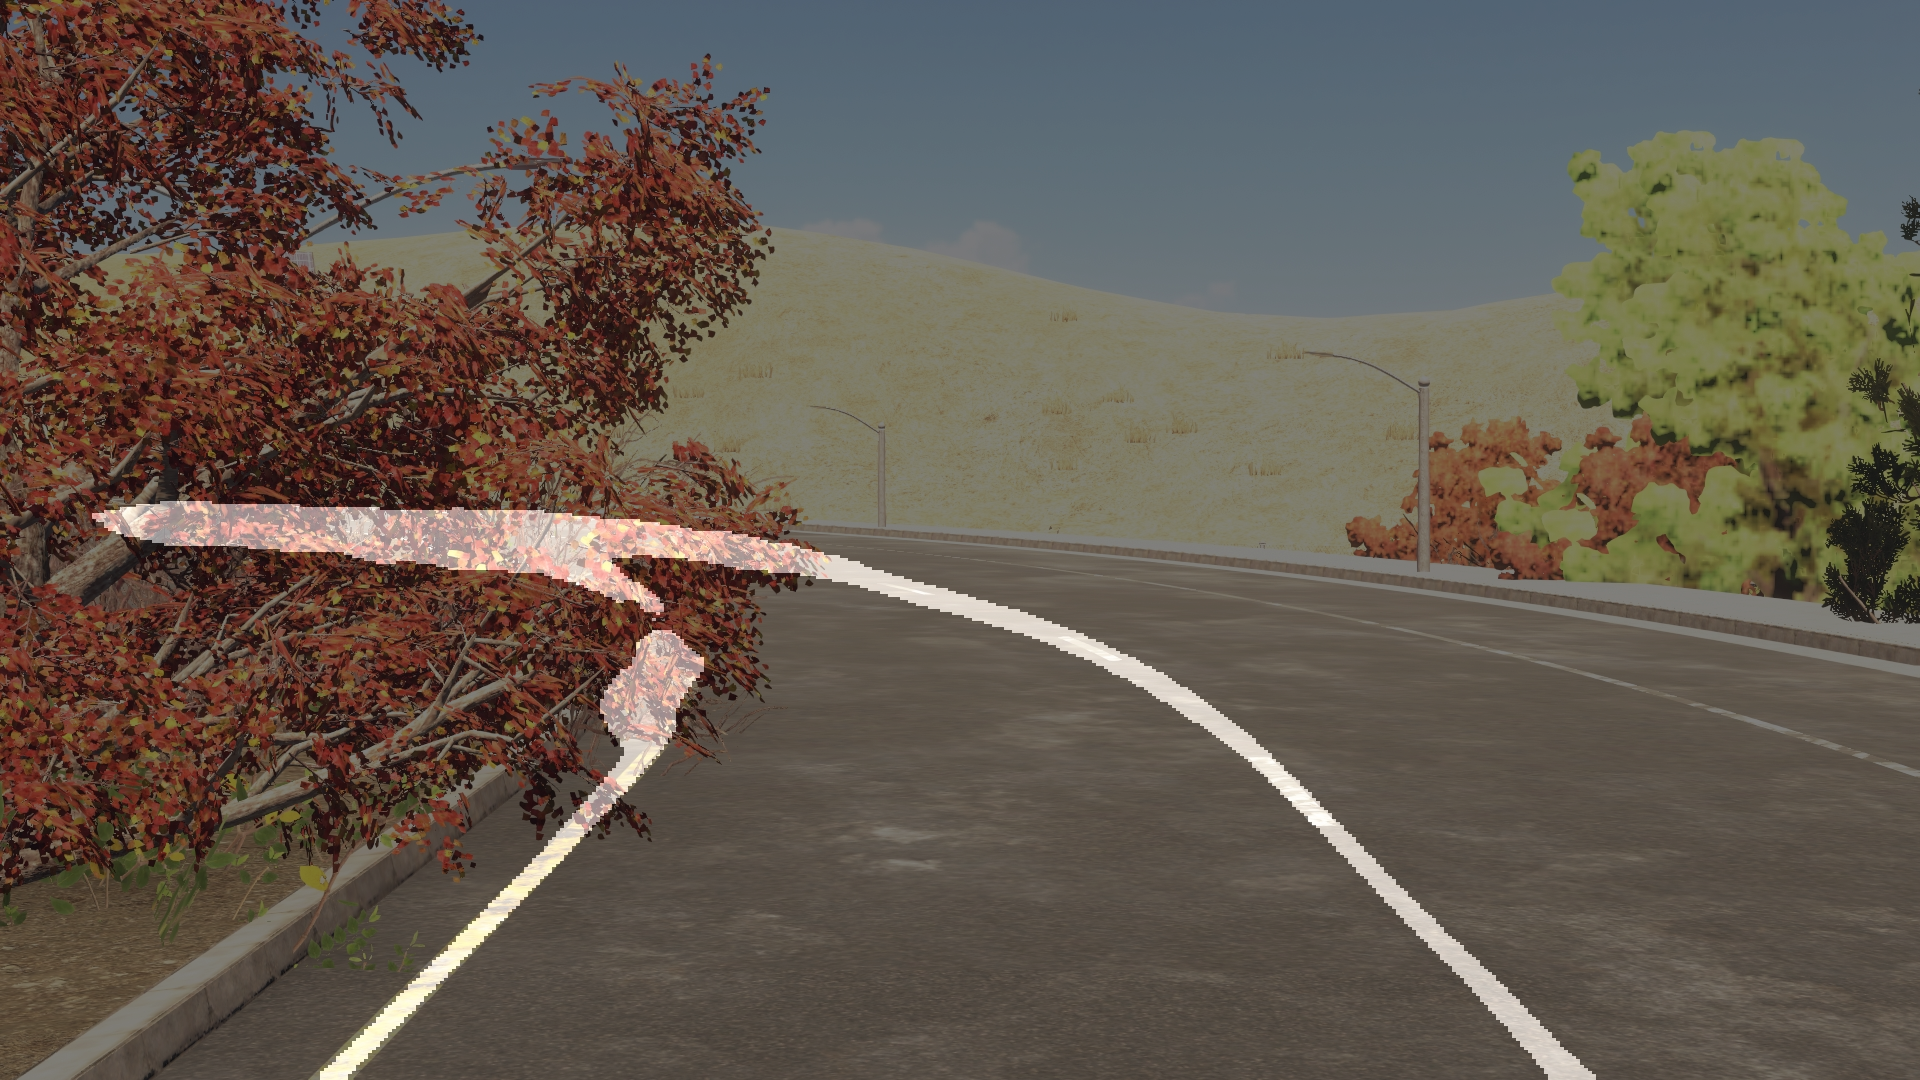
\includegraphics[width=1\linewidth, height=4cm]{images/binseg_ce_resa.png} 
        \caption{}
        \label{fig:subim1}
        \end{subfigure}
        \begin{subfigure}{0.4\textwidth}
        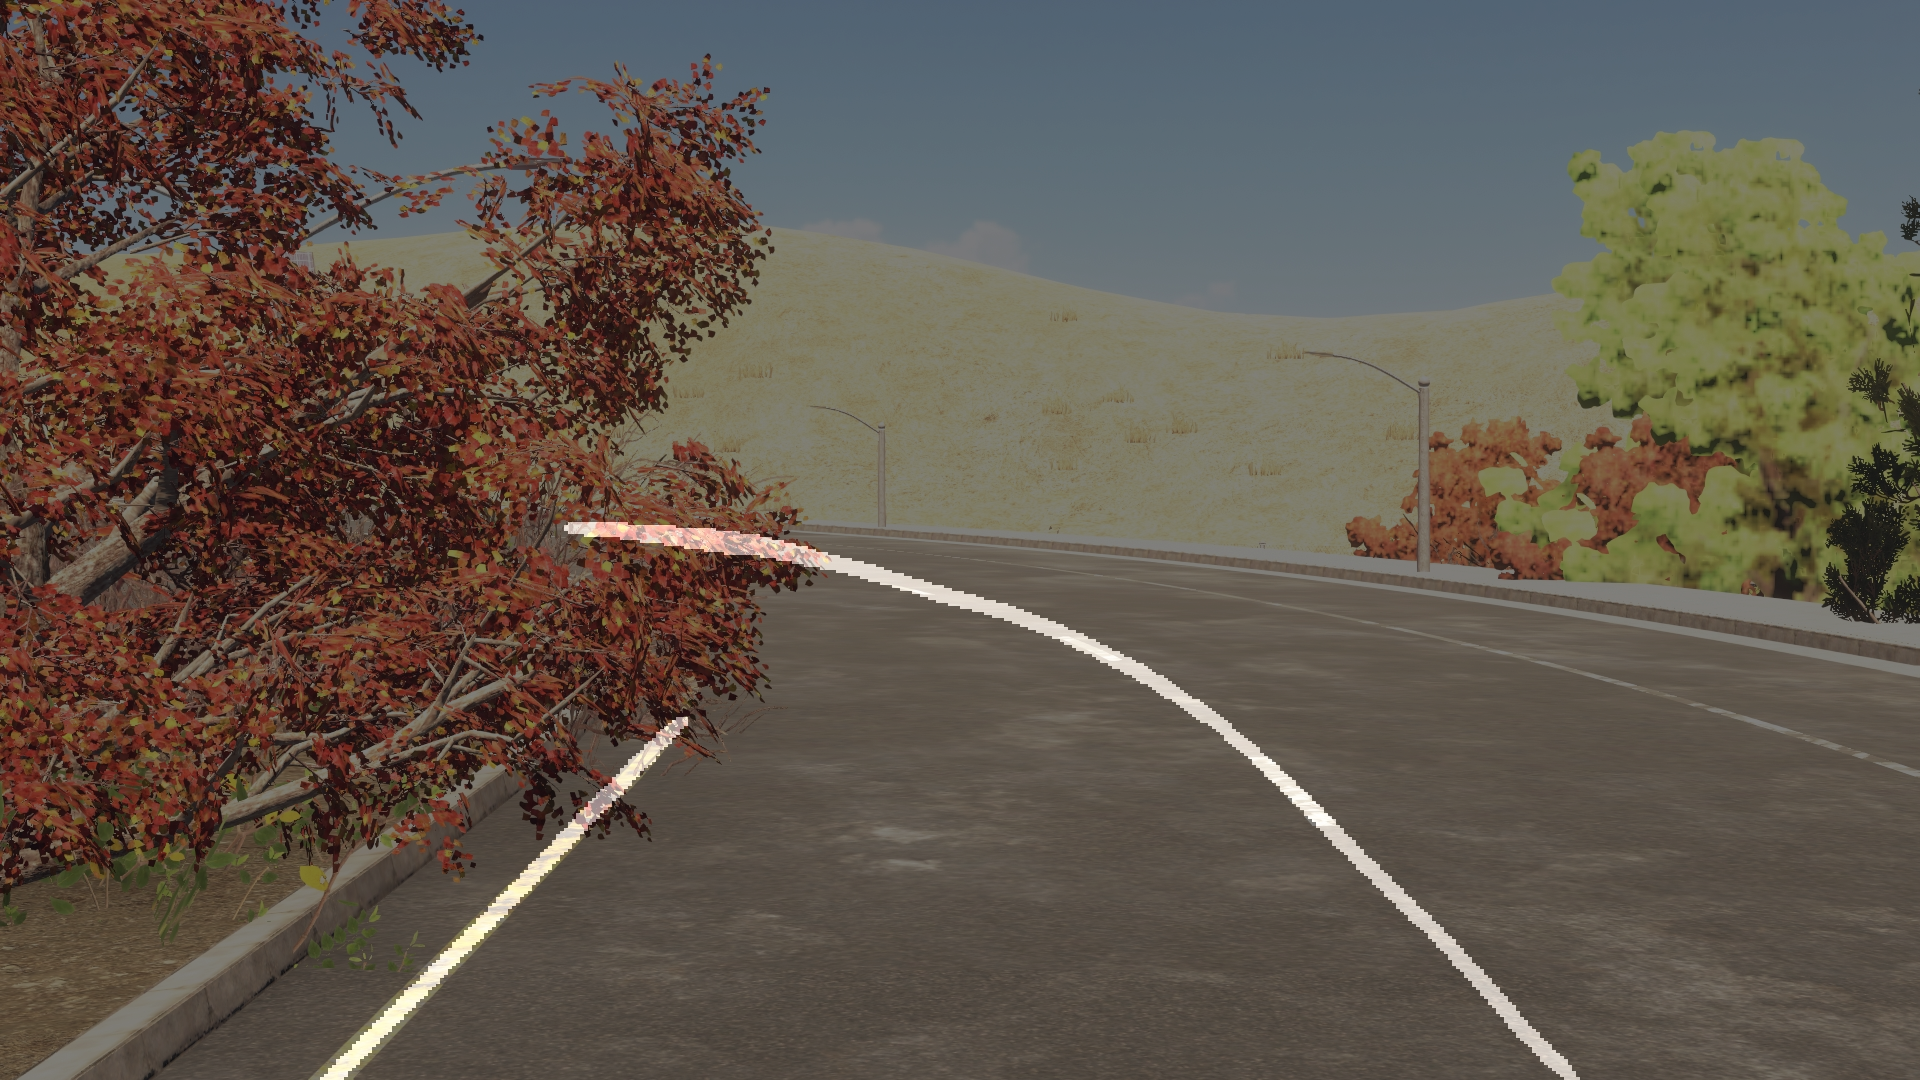
\includegraphics[width=1\linewidth,height=4cm]{images/binseg_dice_resa.png}
        \caption{}
        \label{fig:subim2}
        \end{subfigure}
        \begin{subfigure}{0.4\textwidth}
        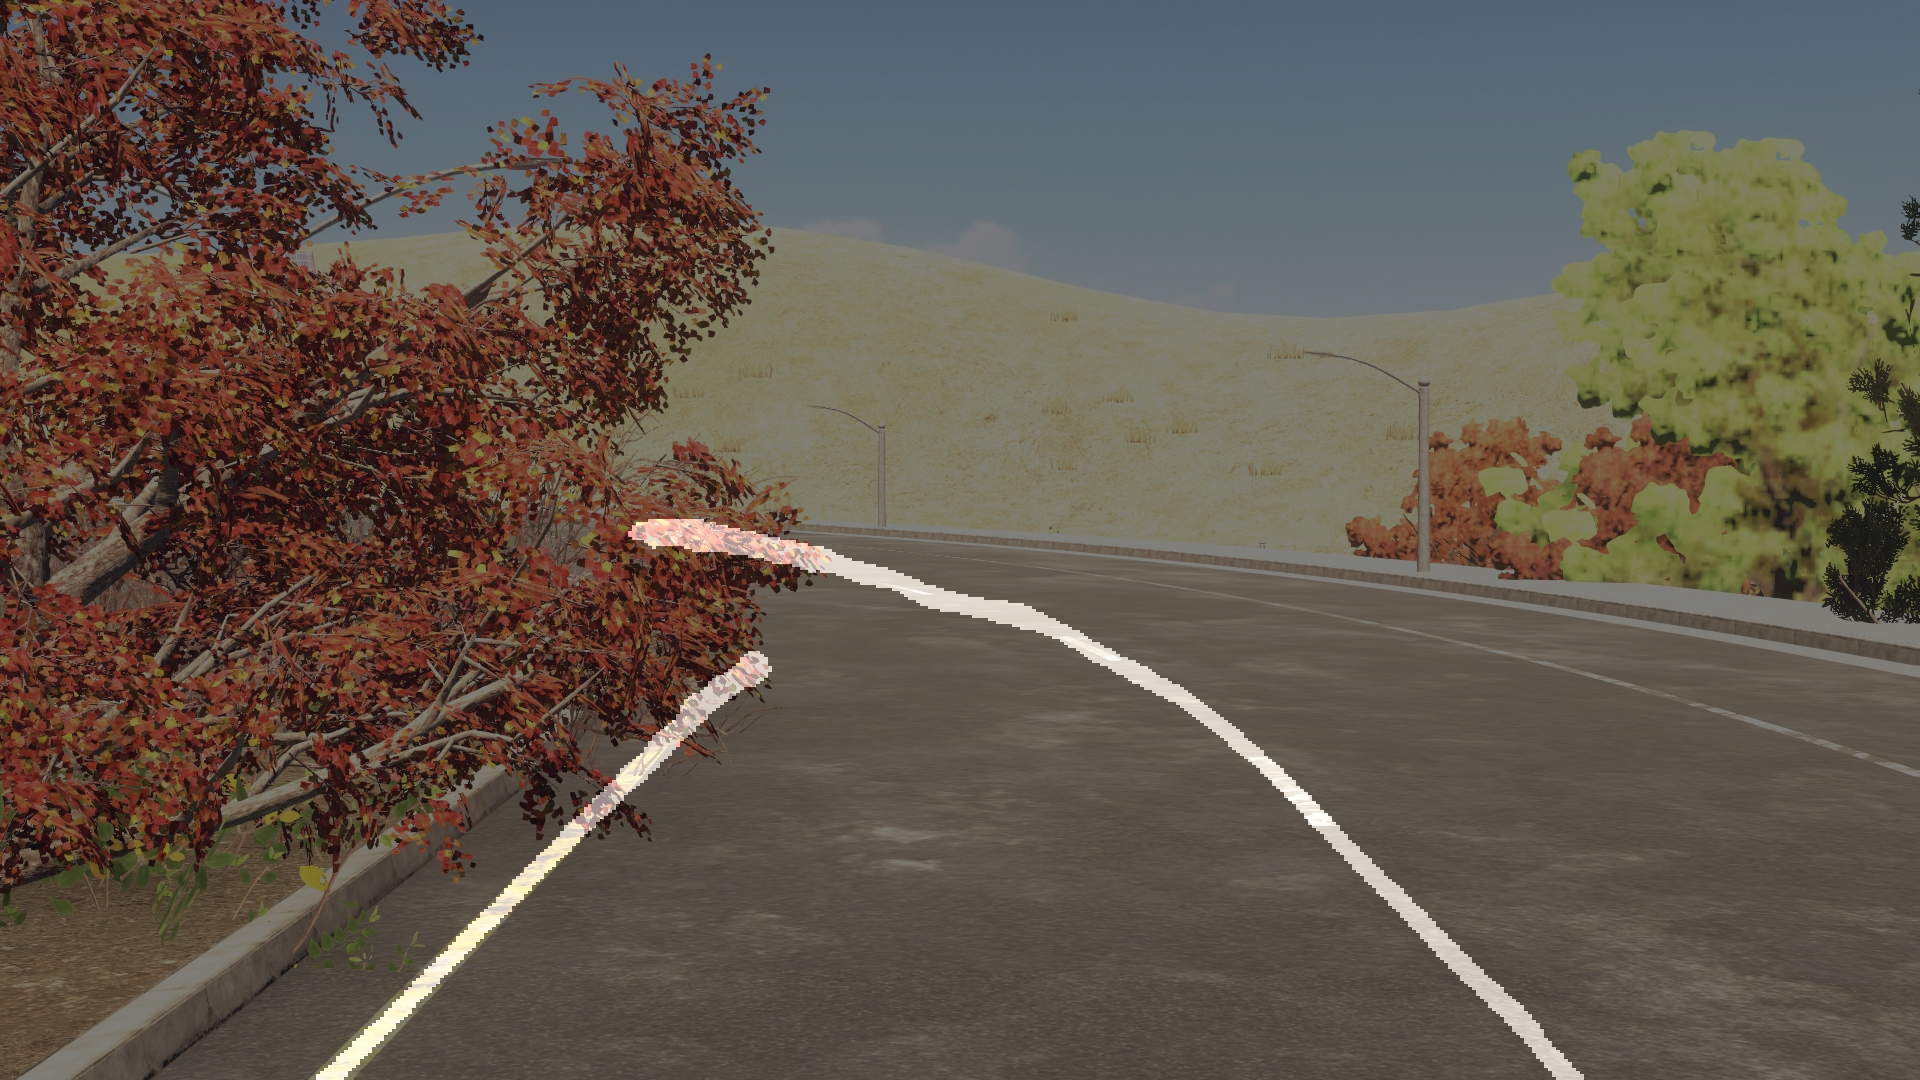
\includegraphics[width=1\linewidth, height=4cm]{images/binseg_focal_resa.png}
        \caption{}
        \label{fig:subim2}
        \end{subfigure}
        \label{fig:image2}
        \end{figure}
    
     \begin{figure}[h]
       \caption{IoU for binary lane segmentation trained on sim3D dataset with cross entropy, dice and focal loss.}
        \centering
        \begin{subfigure}{0.6\textwidth}
        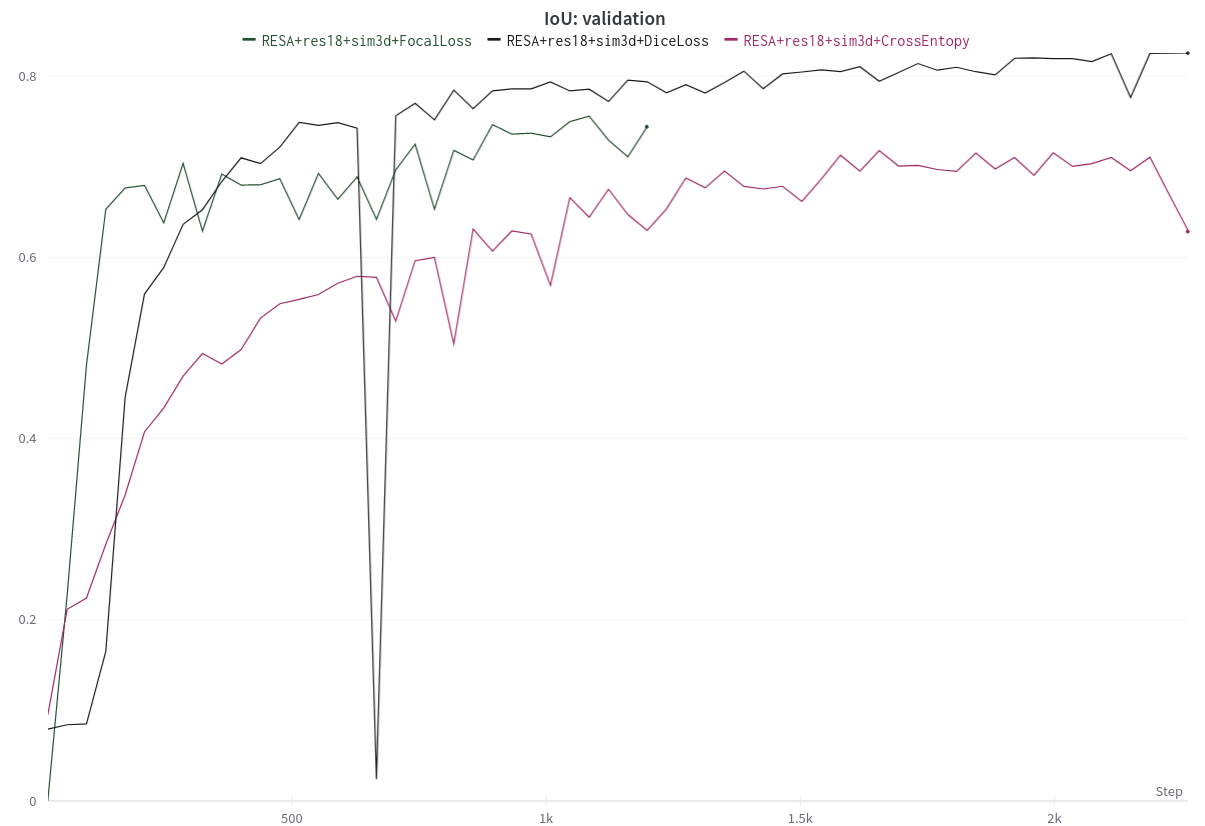
\includegraphics[width=1\linewidth, height=5cm]{images/binseg_IOU.png} 
        \label{fig:subim1}
        \end{subfigure}
        \end{figure}
    
    From Table 5.3 and figure 5.3 we can conclude that using dice loss and focal loss the class imbalance problem is addressed, resulting better in IoU. Moreover there is significant change in the quality of binary lane segmentation.
        After countering the class imbalance problem we trained some models on sim3d dataset which predicts binary lane segmentation for all the lanes present in the scene.
        
        
           \begin{table}[h!]
    \caption{Quantitative results for binary lane segmentation on sim3D dataset for all the lanes present in the scene}
    \centering
    \begin{tabular}{|l|l|l|}
    \hline
        \textbf{Method} & \textbf{IoU} & \textbf{FPS} \\ \hline
        SCNN(Res18+Focal Loss) & 44.01 & $\approx$ \textbf{70} \\\hline
        RESA(Res18+Dice Loss) & 86.56 & $\approx$ 55 \\\hline
        RESA(Res50+Dice Loss) & \textbf{86.67} & $\approx$ 50 \\\hline
    \end{tabular}
\end{table}
        
        
        \begin{figure}[h]
       \caption{IoU for binary lane segmentation trained on sim3D dataset with cross entropy, dice and focal loss.}
        \centering
        \begin{subfigure}{0.6\textwidth}
        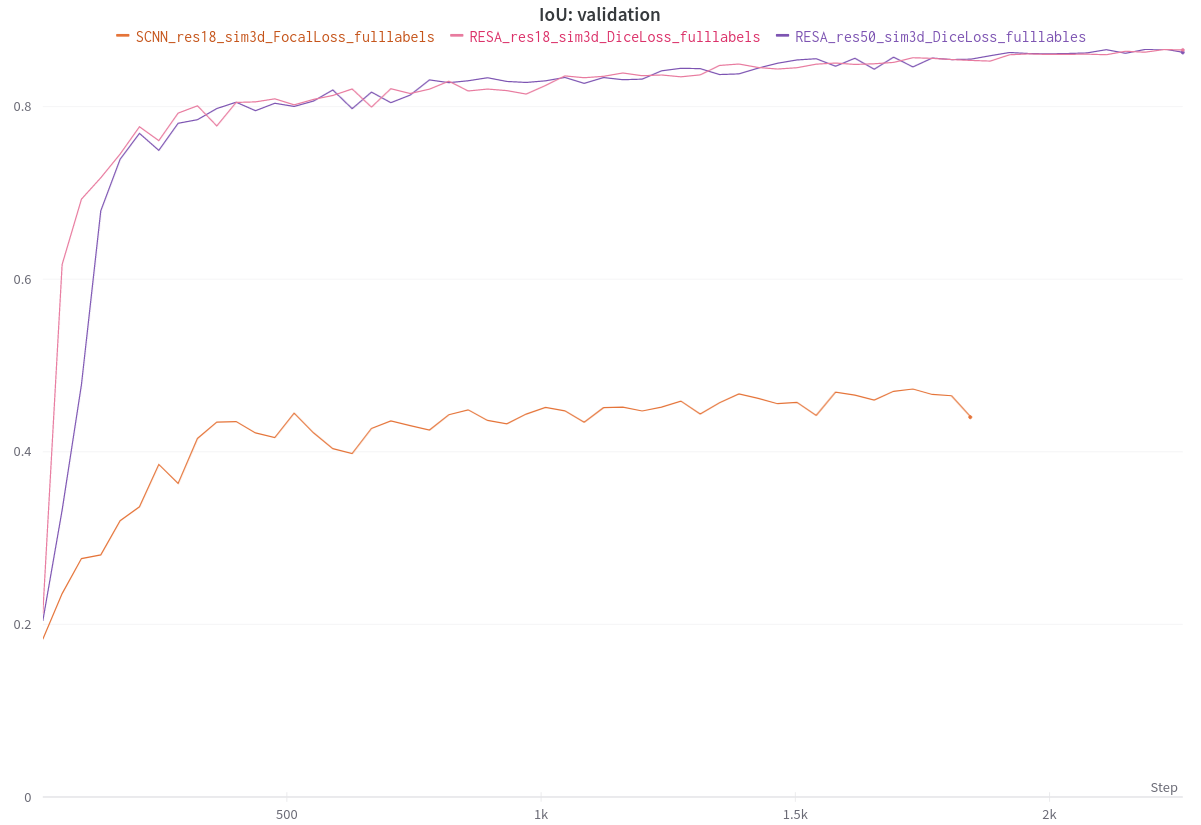
\includegraphics[width=1\linewidth, height=5cm]{images/IOU_full.png} 
        \label{fig:subim1}
        \end{subfigure}
        \end{figure}
        
        
        \begin{figure}[h]
       \caption{Qualitative results for binary lane segmentation trained on sim3d dataset for all the lanes present in the scene: (a) SCNN(Res18+Focal Loss) (b) RESA(Res18+Dice Loss) (c)RESA(Res18+Focal Loss)}
        \centering
        \begin{subfigure}{0.4\textwidth}
        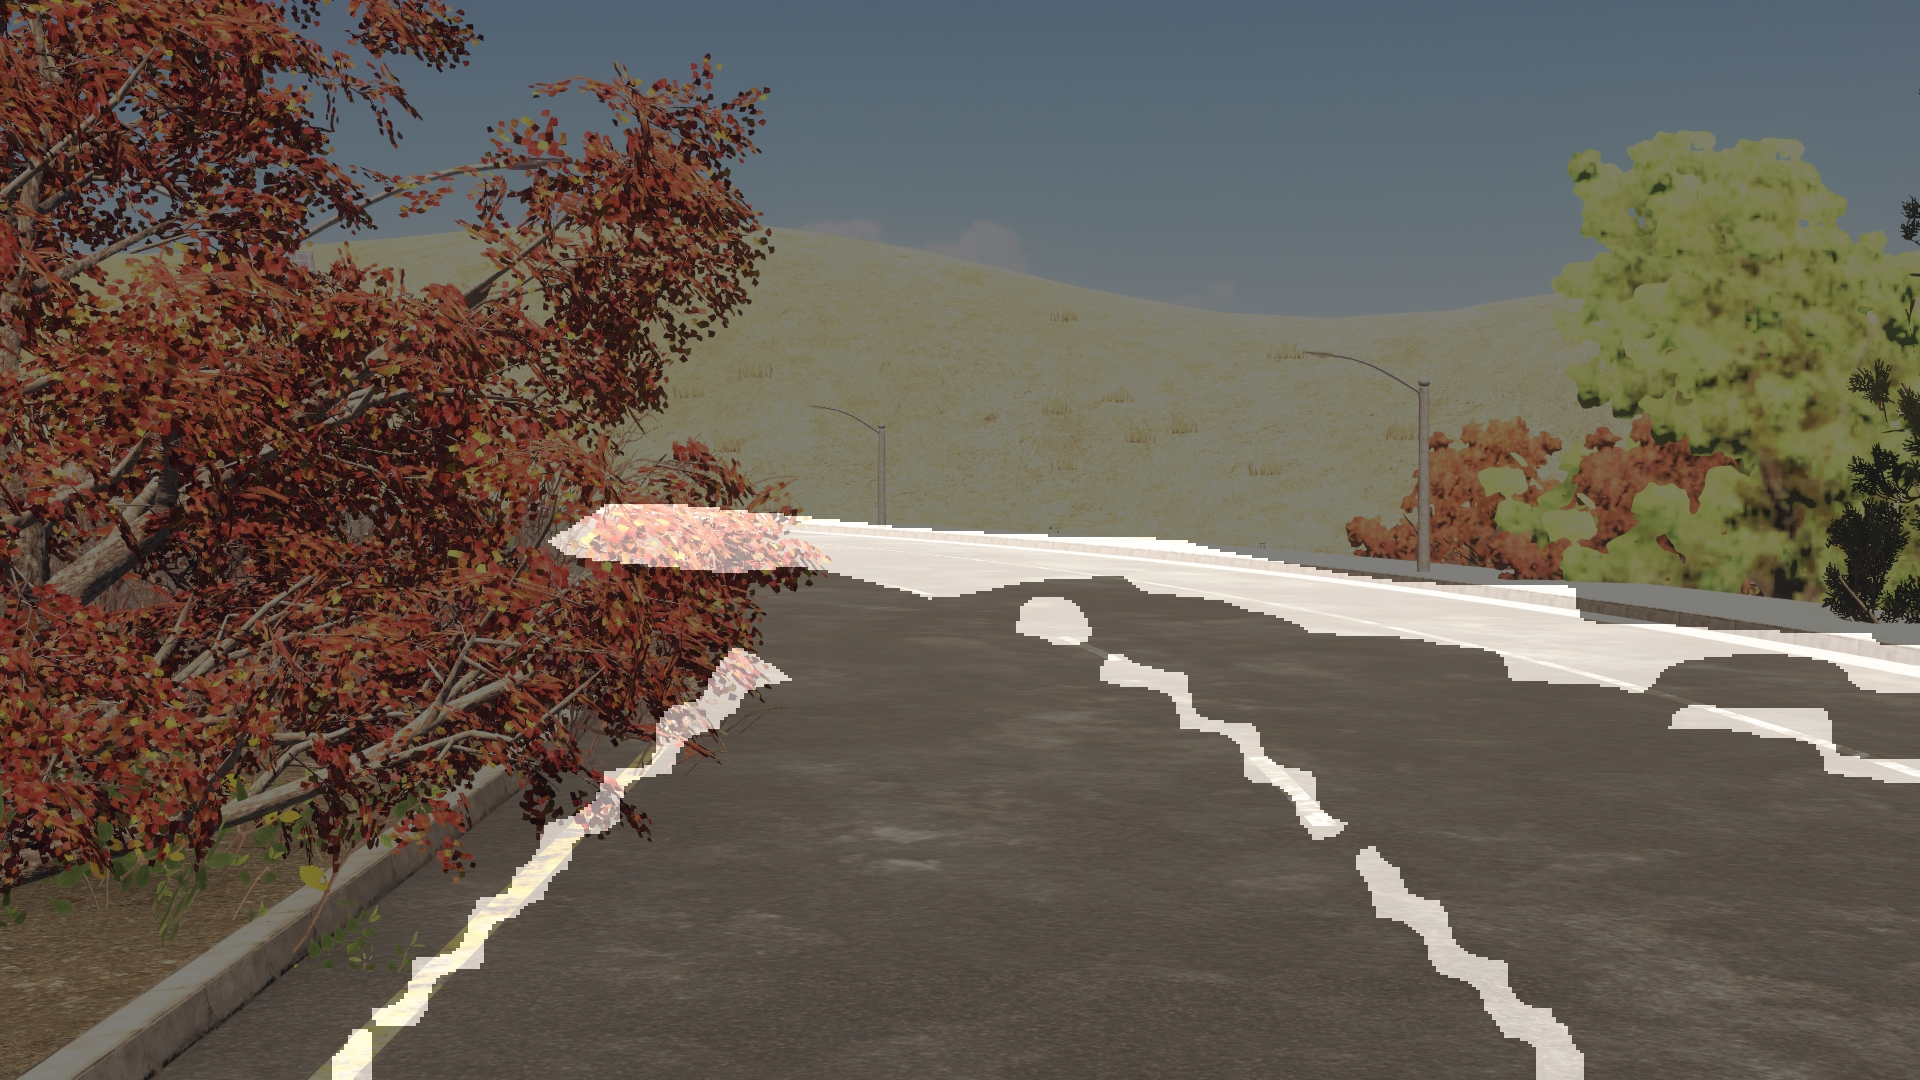
\includegraphics[width=1\linewidth, height=4cm]{images/full_res18_scnn_focal.png} 
        \caption{}
        \label{fig:subim1}
        \end{subfigure}
        \begin{subfigure}{0.4\textwidth}
        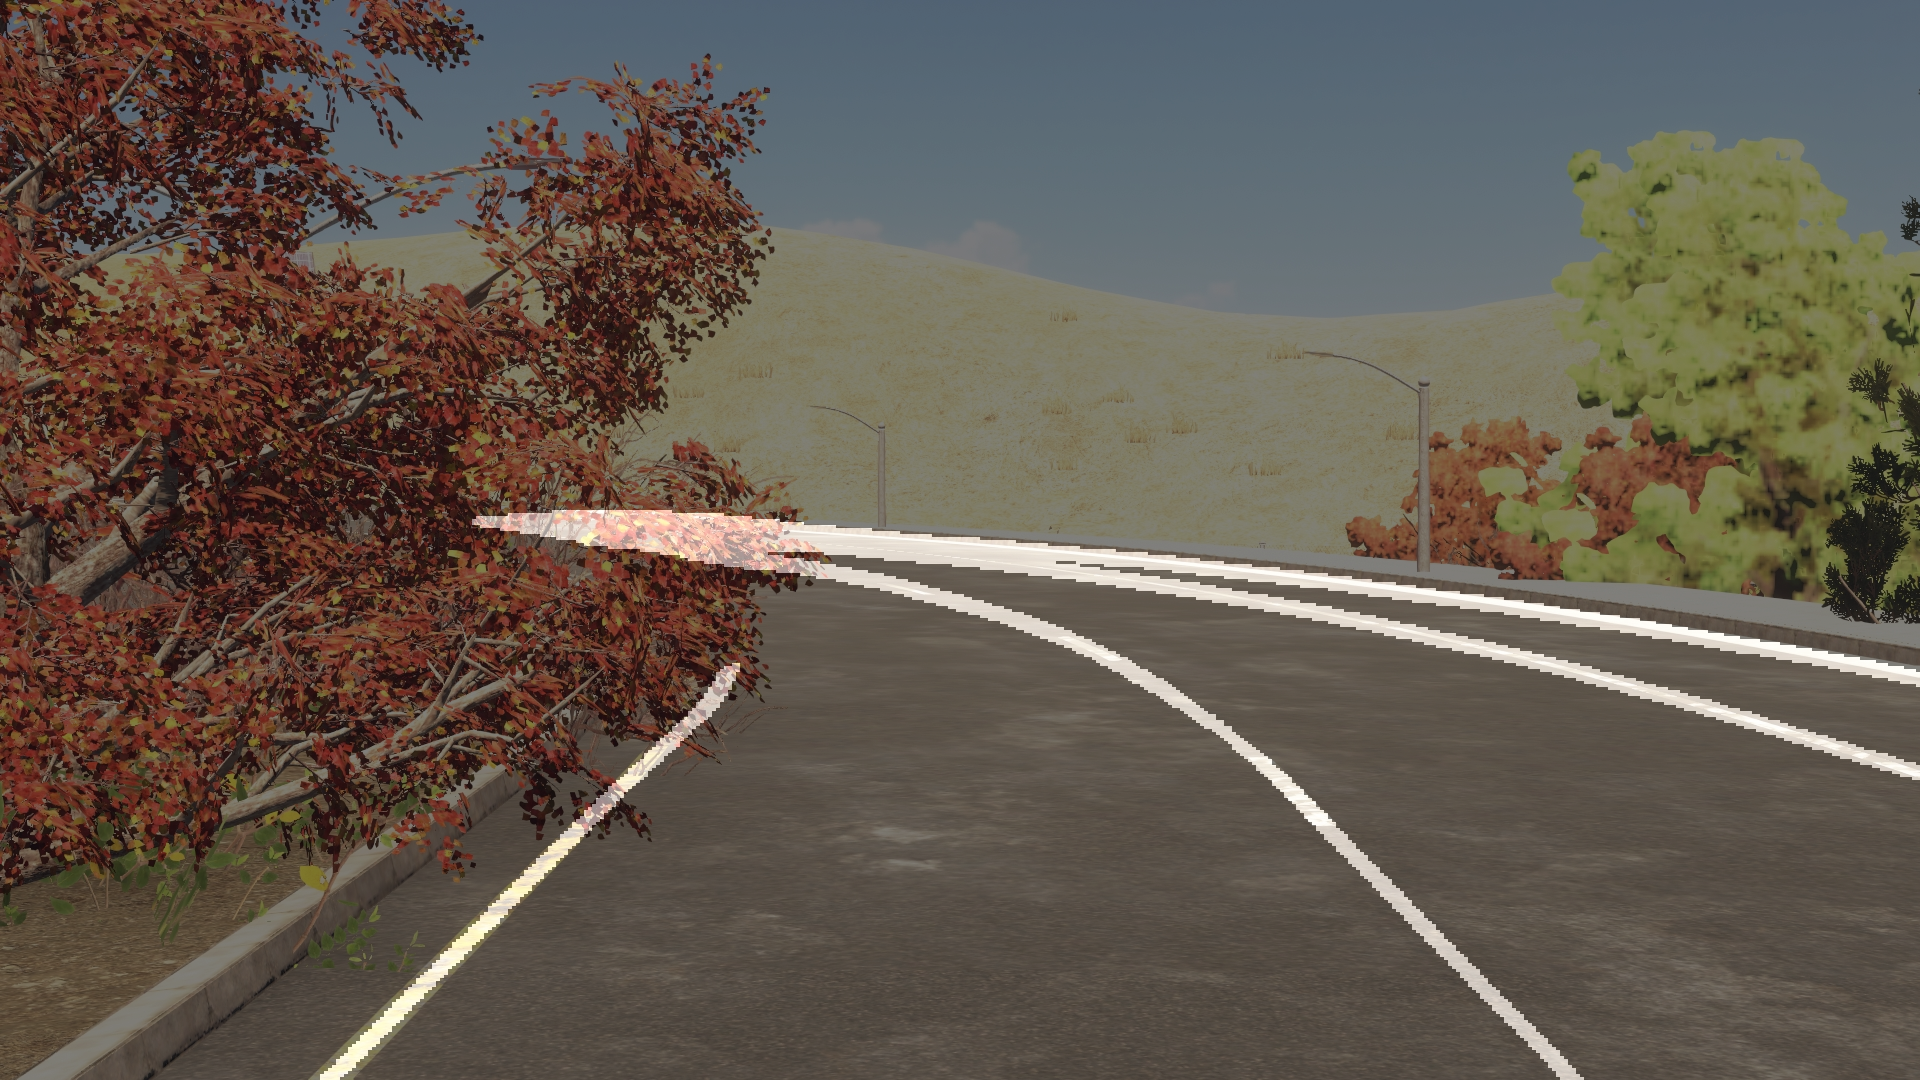
\includegraphics[width=1\linewidth,height=4cm]{images/Resa_r18_full_dice.png}
        \caption{}
        \label{fig:subim2}
        \end{subfigure}
        \begin{subfigure}{0.4\textwidth}
        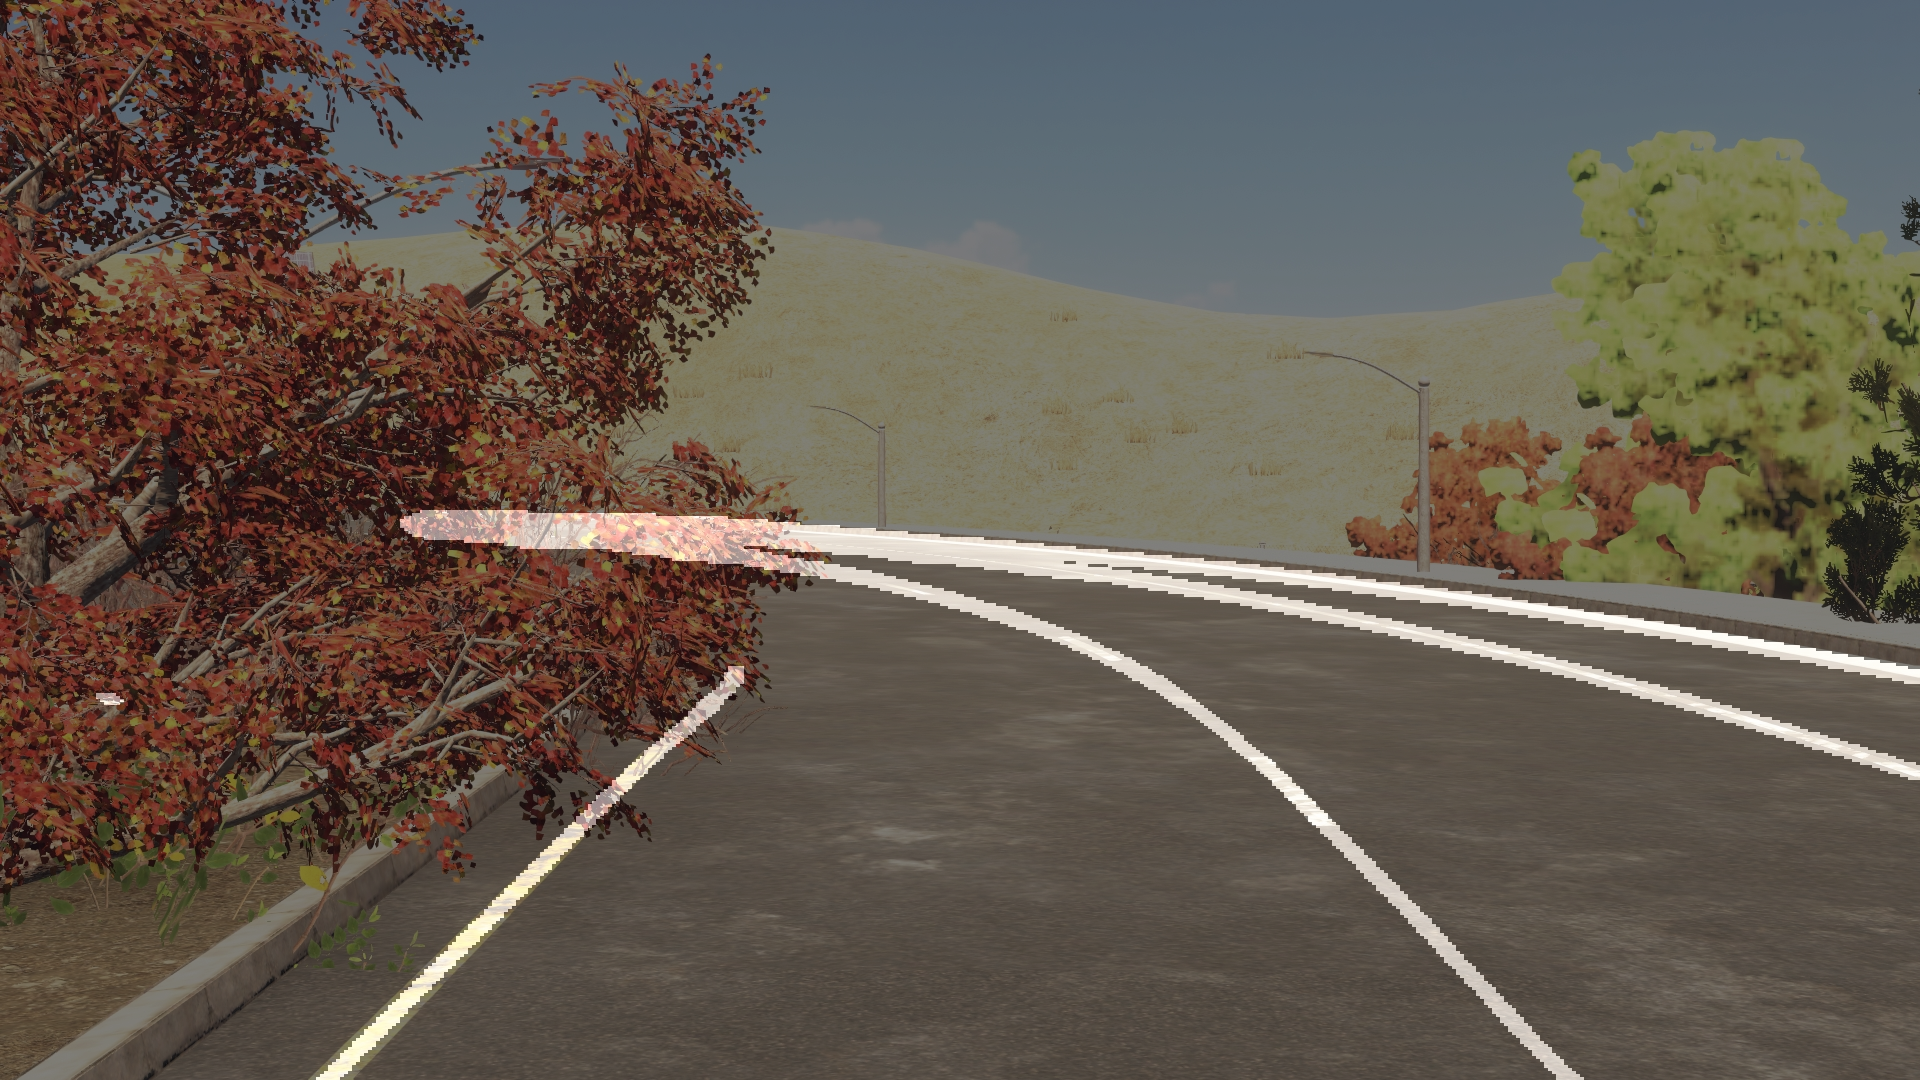
\includegraphics[width=1\linewidth, height=4cm]{images/Resa_r50_full_dice.png}
        \caption{}
        \label{fig:subim2}
        \end{subfigure}
        \label{fig:image2}
        \end{figure}
        
    
    
        %---------------------------------------------------------------------%
    \section{3D Lane Detection}
    
    \subsubsection{Approach: 1}
    \subsubsection{Approach: 2}
    
    
    

    \textbf{Discuss about the struggles with the dataset and how you have over come it} 
        
    \begin{itemize}
        \item Class imbalance ----->  Class weighting CCE -----> Focal Loss ----> Dice Loss
    \end{itemize}
      


\begin{itemize}
     \item Discuss here quantativelly qualitatively along with scientific arguments what you have done and how you have improved your results for 2d lane detection (class imbalance).
\end{itemize}
     \begin{table}[h]
    \caption{Focal and Dice loss and analyze the results qualitatively too here all trained on sim3d only trained with egovehicle lanes for segmentation \textbf{Add all the difference in qualitative results and the IOU graph}}
    \centering
    \begin{tabular}{|l|l|l|}
    \hline
        \textbf{Method} & \textbf{IoU} & \textbf{FPS} \\ \hline
        RESA(Res18+Cross Entropy) & 71.79 & $\approx$ 45 \\ \hline
        SCNN(Res18+Cross Entropy) & 44.12 & $\approx$ 70  \\ \hline
        RESA(Res50+Cross Entropy) & 74.11 & $\approx$ 40  \\ \hline
        RESA(Res18+Focal Loss) & 75.59 & $\approx$ 55 \\\hline
        RESA(Res18+Dice Loss) & 82.57 & $\approx$ 50 \\\hline
        RESA(Res50+Dice Loss) & 83.33 & $\approx$ 50 \\\hline
    \end{tabular}
\end{table}
    
    
     \begin{table}[h]
    \caption{FULL label lane segmentation results with dice and focal loss \textbf{Add all the difference in qualitative results and the IOU graph}}
    \centering
    \begin{tabular}{|l|l|l|}
    \hline
        \textbf{Method} & \textbf{IoU} & \textbf{FPS} \\ \hline
        SCNN(Res18+Focal Loss) & 44.01 & $\approx$ 70 \\\hline
        RESA(Res18+Dice Loss) & 86.56 & $\approx$ 55 \\\hline
        RESA(Res50+Dice Loss) & 86.67 & $\approx$ 50 \\\hline
    \end{tabular}
\end{table}

    \section{Use case 1}

    Describe results and analyse them
    \begin{itemize}
        \item \textbf{Balanced Scenes}
    \end{itemize}

    \begin{table}[htbp]
    \addtolength{\tabcolsep}{-1pt}
    \begin{center}
    \caption{To be filled later}
    \begin{tabular}{|p{0.3\linewidth}|p{0.1\linewidth}|p{0.1\linewidth}|p{0.1\linewidth}|p{0.1\linewidth}|p{0.1\linewidth}|p{0.1\linewidth}|}
    \hline
        \textbf{Method} & \textbf{AP} & \textbf{F-Score} & \textbf{x error near(m)} & \textbf{x error far(m)} & \textbf{z error near(m)} & \textbf{z error far(m)} \\ \hline
        Gen-LaneNet & 90.1 & 88.1 & 0.061 & 0.496 & 0.012 & 0.214 \\ \hline
        3D LaneNet & 89.3 & 86.4 & 0.068 & 0.477 & 0.015 & \textbf{0.202} \\ \hline
        CLGo & \textbf{94.2} &\textbf{ 91.9} & 0.061 & \textbf{0.361} & 0.029 & 0.250 \\ \hline
        3D-LaneNet(1/att) &  93.2 & 91.0 & 0.082 & 0.439 & \textbf{0.011} & 0.242 \\ \hline
        Gen-LaneNet(1/att) & 92.4 & 90.3 & 0.080 & 0.473 & \textbf{0.011} & 0.247 \\ \hline
        Gen-LaneNet(RESA+Res18) & 91.8 & 89.7 & \textbf{0.06} & 0.466 & 0.0114 & 0.24 \\ \hline
        Gen-LaneNet(RESA+Res50) & 92.2 & 90.2 &\textbf{ 0.06} & 0.461 & 0.0122 & 0.24 \\ \hline
    \end{tabular}
    \end{center}
\end{table}

    \begin{itemize}
        \item \textbf{Rarely Observed}
    \end{itemize}
    
        \begin{table}[htbp]
    \centering
    \caption{To be filled later}
    \begin{tabular}{|p{0.3\linewidth}|p{0.1\linewidth}|p{0.1\linewidth}|p{0.1\linewidth}|p{0.1\linewidth}|p{0.1\linewidth}|p{0.1\linewidth}|}
    \hline
        \textbf{Method} & \textbf{AP} & \textbf{F-Score} & \textbf{x error near(m)} & \textbf{x error far(m)} & \textbf{z error near(m)} & \textbf{z error far(m)} \\ \hline
        Gen-LaneNet & 79.0 & 78.0 & 0.139 & 0.903 & 0.030 & 0.539 \\ \hline
        3D LaneNet & 74.6 & 72.0 & 0.166 & 0.855 & 0.039 &\textbf{ 0.521} \\ \hline
        CLGo &\textbf{ 88.3} &\textbf{ 86.1} & 0.147 & \textbf{0.735} & 0.071 & 0.609 \\ \hline
        3D-LaneNet(1/att) & 85.8 & 84.1 & 0.289 & 0.925 &\textbf{ 0.025} & 0.625 \\ \hline
        Gen-LaneNet(1/att) & 83.2 & 81.7 & 0.283 & 0.915 & 0.028 & 0.653 \\ \hline
        Gen-LaneNet(RESA+Res18) &  84.9 & 83.2 &\textbf{ 0.135} & 0.886 & 0.0308 & 0.607 \\ \hline
        Gen-LaneNet(RESA+Res50) & 83.7 & 82.3 & 0.14 & 0.919 & 0.0283 & 0.604 \\ \hline
    \end{tabular}
\end{table}

  \begin{itemize}
        \item \textbf{Visual Variations}
    \end{itemize}
    
        \begin{table}[htbp]
    \centering
    \caption{To be filled later}
    \begin{tabular}{|p{0.3\linewidth}|p{0.1\linewidth}|p{0.1\linewidth}|p{0.1\linewidth}|p{0.1\linewidth}|p{0.1\linewidth}|p{0.1\linewidth}|}
    \hline
        \textbf{Method} & \textbf{AP} & \textbf{F-Score} & \textbf{x error near(m)} & \textbf{x error far(m)} & \textbf{z error near(m)} & \textbf{z error far(m)} \\ \hline
        Gen-LaneNet & 87.2 & 85.3 & 0.074 & 0.538 & 0.015 & 0.232 \\ \hline
        3D LaneNet & 74.9 & 72.5 & 0.115 & 0.601 & 0.032 & \textbf{0.230} \\ \hline
        CLGo & 89.2 & 87.3 & 0.084 & \textbf{0.464} & 0.045 & 0.312 \\ \hline
        3D-LaneNet(1/att) & 87.4 & 85.4 & 0.118 & 0.559 & 0.018 & 0.290 \\ \hline
        Gen-LaneNet(1/att) & 88.5 & 86.8 & 0.104 & 0.544 & 0.016 & 0.294 \\ \hline
        Gen-LaneNet(RESA+Res18) & \textbf{ 91.1} &\textbf{ 89.2} & 0.734 & 0.496 & \textbf{0.0134} & 0.259 \\ \hline
        Gen-LaneNet(RESA+Res50) & 90.7 & 88.8 & \textbf{0.0653} & 0.477 & 0.014 & 0.258 \\ \hline
    \end{tabular}
\end{table}
    \section{Use case 2}

    \section{Use case 3}
\end{document}
